\documentclass[12pt]{article}
\usepackage{amsmath}
\usepackage{amsfonts}
\usepackage{amssymb}
\usepackage{setspace}
\usepackage{mathtools}
\usepackage{graphicx}
\usepackage{hyperref}
\graphicspath{ {figures/} }
\usepackage{tikz}
\usepackage[margin=0.7in]{geometry}
\usepackage{fancyhdr}
	%\thispagestyle{fancy}
	
 \begin{document}

\newenvironment{myspace}[1]
	{\begin{spacing}{#1}}
	{\end{spacing}}

%----------------------------------------------------------------------------------------
%	TITLE PAGE
%----------------------------------------------------------------------------------------

\begin{titlepage} % Suppresses displaying the page number on the title page and the subsequent page counts as page 1
	\newcommand{\HRule}{\rule{\linewidth}{0.5mm}} % Defines a new command for horizontal lines, change thickness here
	
	\center % Centre everything on the page
	
	%------------------------------------------------
	%	Headings
	%------------------------------------------------
	
	\textsc{\LARGE Illinois Institute of Technology}\\[1.5cm] % Main heading such as the name of your university/college
	
	\textsc{\Large CS 425}\\[0.5cm] % Major heading such as course name
	
	\textsc{\large Database Organization}\\[0.5cm] % Minor heading such as course title
	
	%------------------------------------------------
	%	Title
	%------------------------------------------------
	
	\HRule\\[0.4cm]
	
	{\huge\bfseries CS425 Project: Online Distribution Center}\\[0.4cm] % Title of your document
	
	\HRule\\[1.5cm]
	
	%------------------------------------------------
	%	Author(s)
	%------------------------------------------------
	
	\begin{minipage}{0.4\textwidth}
		\begin{flushleft}
			\large
			\textit{Authors}\\
			Hector \textsc{Hernandez}\\
			Ramir \textsc{Aguilos}\\
			Rafael \textsc{Zavala}\\
			Hauyu \textsc{Wang}\\
		\end{flushleft}
	\end{minipage}
	~
	\begin{minipage}{0.4\textwidth}
		\begin{flushright}
			\large
			\textit{Professor}\\
			Dr. Omar \textsc{Aldawud} % Supervisor's name
		\end{flushright}
	\end{minipage}
	
	% If you don't want a supervisor, uncomment the two lines below and comment the code above
	%{\large\textit{Author}}\\
	%John \textsc{Smith} % Your name
	
	%------------------------------------------------
	%	Date
	%------------------------------------------------
	
	\vfill\vfill\vfill % Position the date 3/4 down the remaining page
	
	{\large February 28, 2018} % Date, change the \today to a set date if you want to be precise
	
	%------------------------------------------------
	%	Logo
	%------------------------------------------------
	
	%\vfill\vfill
	%\includegraphics[width=0.2\textwidth]{placeholder.jpg}\\[1cm] % Include a department/university logo - this will require the graphicx package
	 
	%----------------------------------------------------------------------------------------
	
	\vfill % Push the date up 1/4 of the remaining page
	
\end{titlepage}




\begin{myspace}{1.7}
        
\section*{Introduction}  
This project consist of a web solution for an e-commerce application. The project itself will be conducted using a waterfall model \cite{waterfall} for development. The web application will be developed
using JDBC as a back-end and Node.js, html, CSS as a front-end

%*********************************************************************************************
%*********************************************************************************************
%
%					Introduction
%
%*********************************************************************************************
%*********************************************************************************************
\pagebreak
\section*{Requirements}  



%*********************************************************************************************
%*********************************************************************************************
%
%				       Design
%
%*********************************************************************************************
%*********************************************************************************************



\pagebreak
\section*{Design}


%*********************************************************************************************
%*********************************************************************************************
%
%				       Design
%
%*********************************************************************************************
%*********************************************************************************************
\subsection*{Entity Relationship Diagram}
\begin{center}
          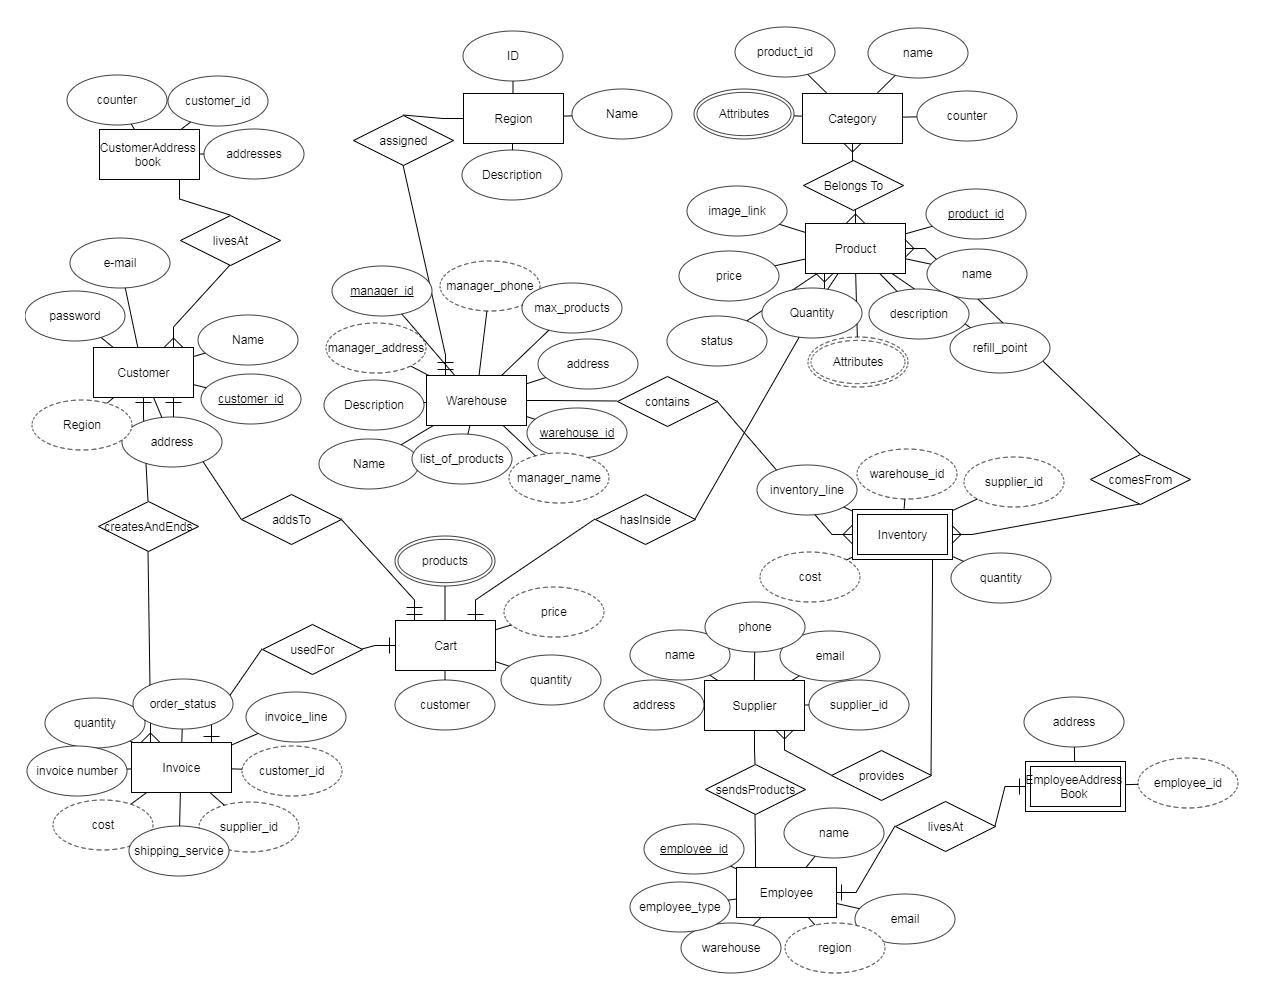
\includegraphics[ height=21cm]{ERD} %width=xxcm
\end{center}
\pagebreak
\section*{Implementation}


%*********************************************************************************************
%*********************************************************************************************
%
%				    Implementation
%
%*********************************************************************************************
%*********************************************************************************************
\pagebreak
\section*{Verification}






%*********************************************************************************************
%*********************************************************************************************
%
%				     Verification
%
%*********************************************************************************************
%*********************************************************************************************
\pagebreak
\section*{Maintenance}  





%*********************************************************************************************
%*********************************************************************************************
%
%				     Maintenance
%
%*********************************************************************************************
%*********************************************************************************************
\pagebreak
\section*{Conclusions}  





%*********************************************************************************************
%*********************************************************************************************
%
%					END
%
%*********************************************************************************************
%*********************************************************************************************
\pagebreak
\begin{thebibliography}{9}
\bibitem{waterfall}
   \textit{Waterfall Model and Testing Methodology}\\
   \url{https://www.guru99.com/testing-methodology.html#2}

\end{thebibliography}
  
\end{myspace}
\end{document}
